\documentclass{article}

\usepackage[russian]{babel}    %enable russian languge
\usepackage[utf8]{inputenc}
\usepackage[T2A]{fontenc}

\usepackage[a4paper, includefoot, 
            left=1.0cm, right=1.0cm, 
            top=1.5cm, bottom=1.5cm, 
            headsep=1cm, footskip=1cm]{geometry}
\usepackage{amsmath}
\usepackage{amssymb}
\usepackage{array}
\usepackage{caption}
\usepackage{longtable}
\usepackage{multirow}

\pagestyle{plain}

\usepackage{graphicx}
\graphicspath{{pics/}}

\usepackage[fontsize=12]{scrextend}
\renewcommand{\baselinestretch}{1.5}


%%%%%%%%%%%%%%%%%%%%%%%%%%%%%%%%%%%%%%%%%%%%%%%%%%%%%%%%%%%%%%%%%%%
%                        My commands                              %
%%%%%%%%%%%%%%%%%%%%%%%%%%%%%%%%%%%%%%%%%%%%%%%%%%%%%%%%%%%%%%%%%%%
\newcommand{\n}{\vspace{\baselineskip}}
\newcommand{\ntb}{\tabularnewline}
\newcommand{\tabscale}[1]{\renewcommand{\arraystretch}{#1}}

% \pich{scale}{pic}{caption}
\newcommand{\pic}[3]
{
\noindent
\begin{minipage}{\linewidth}
  \center{\includegraphics[width = #1\linewidth]{#2}}
  \captionof{figure}{#3}
\end{minipage}
}

% \pich{scale}{minipage height}{pic}{caption}
\newcommand{\pich}[4]
{
\noindent
\begin{minipage}{\linewidth}
  \center{\includegraphics[width = #1\linewidth, height = #2]{#3}}
  \captionof{figure}{#4}
\end{minipage}
}
%%%%%%%%%%%%%%%%%%%%%%%%%%%%%%%%%%%%%%%%%%%%%%%%%%%%%%%%%%%%%%%%%%%%


\begin{document}

\begin{center}{
\normalsize Санкт-Петербургский Государственный Политехнический университет\\
Институт Прикладной Математики и Механики\\
[7cm]
} 
\Huge Отчет\\ 
\large по вычислительной лабораторной работе:\\
\large	
\textbf{"Расчет пограничного слоя, развивающегося на плоской пластине."} \\
[5cm]
\begin{flushleft}
\quad\quad Выполнил:  \hspace{10 cm} \parbox[t]{4.5cm}{Пинаев И. А. \\ студент гр.33601/1 }\\
\end{flushleft}
\vfill
{\large Санкт-Петербург \\ 2014} 
\end{center}
\thispagestyle{empty}

%\begin{center}
%{\LARGE \bf Расчет пограничного слоя, развивающегося на плоской пластине.}
%\end{center}

\section{Задание}
Выполнить  расчет  ламинарного  течения  и  теплообмена  несжимаемой  жидкости,  обтекающей гладкую плоскую пластину. Для динамического пограничного слоя провести анализ влияния типа граничного условия, ставящегося на удалении от стенки, на получаемое решение. Выполнить сопоставление полученных результатов с автомодельным решением уравнений пограничного слоя (задача Блазиуса). Для температурного пограничного слоя провести сопоставление с автомодельным решением для разных значений числа Прандтля. 

\section{Постановка задачи}

\pic{1}{problem.png}{Рассчетная область.}

На рисунке 1 представлена расчетная область $ADFC$: $BC$ -- пластина длиной $L$, $AD$ и $CF$ –- входная и выходная границы, $DF$ –- верхняя граница расчетной области. В расчетную область включен участок $ABED$ выше по потоку, $AB = 0.1L$. На пластину слева набегает однородный поток со скоростью $V$. Течение определяется  одним  безразмерным  параметром – числом  Рейнольдса  $Re = \frac{V \cdot L}{\nu}$,  здесь  $\nu$ -- кинематический коэффициент вязкости. 

Использована одноблочная неравномерная сетка. Высота расчетной области $h = 0.25L$, $BC = L, AB = 0.1L, AD = 0.25$. Количество узлов на ребрах и коэффициенты сгущения могут быть заданы в соответствии со значениями, приведенными в таблице ниже:

\begin{center}
  \begin{tabular}{|p{5cm}|>{\centering}p{3cm}|>{\centering}p{3cm}|>{\centering}p{3cm}|}
  \hline 	
  Сегмент               &   $AD, CF$   & $AB, CD$ & $BC, EF$ \ntb
  \hline 	
  Число узлов           &     31       &  9       & 31       \ntb
  \hline 	
  Коэффициент сгущения  &    1.05      & 0.85     & 1.1      \ntb
  \hline 	
  \end{tabular}
\end{center}

\section{Анализ результатов}
\subsection{Распределение модуля вектора скорости}

\pich{0.9}{3cm}{vel_x.png}{Распределение скорости по оси $Ox$ (symmetry).}

\n
\pich{0.9}{3cm}{vel_x_out.png}{Распределение скорости по оси $Ox$ (outlet).}

\n
\pich{0.9}{3cm}{vel_y.png}{Распределение скорости по оси $Oy$ (symmetry).}

\n
\pich{0.9}{3cm}{vel_y_out.png}{Распределение скорости по оси $Oy$ (outlet).}

На (рис. 1) и (рис. 2) можно видеть, что толщина пограничного слоя увеличивается с удалением от начала пластины. Скорость на пластине принимает минимальное значение и возрастает с координатой $Oy$; вне пограничного слоя скорость принимает максимальное постоянное значение. При граничном условии нормированного давления (рис.2) на врехней границе расчетной области (outlet), толщина пограничного слоя несколько больше, чем при граничном условии симметрии (рис. 1) на верехней границе расчетной области (symmetry). 
\subsection{Распределение давления}

\pich{0.9}{3cm}{press.png}{Давление (symmetry).}
\pich{0.9}{3cm}{press_out.png}{Давление (outlet).}

В обоих случаях граничных условий на границе расчетной области, давление максимально в начале пластины. В случае граничного условия нормированного давления, давление в расчетной области устанавливается на некотором постоянном значении (рис. 7), чего нельзя сказать про случай с граничным условием симметрии (рис. 6).

\subsection{Толщина пограничного слоя}
\subsubsection{Верхняя граница symmetry}

%$\delta \approx \frac{5 \cdot x}{\sqrt{Re_x}}$,  где $Re_x =\frac{ V \cdot x}{\nu}$).
$\delta_{0.99\,\text{эксп.}}$ -- экспериментальная толщина пограничного слоя.\\
$\delta_{0.99\,\text{ан.}}$ -- аналитическая толщина пограничного слоя, полученная при помощи формул

\begin{equation}
\delta \approx \frac{5 \cdot x}{\sqrt{Re_x}},
\quad
Re_x =\frac{ V \cdot x}{\nu}
\end{equation}

\n\n
\noindent
\begin{minipage}{\linewidth}
  \begin{minipage}{0.5\linewidth}
    \center{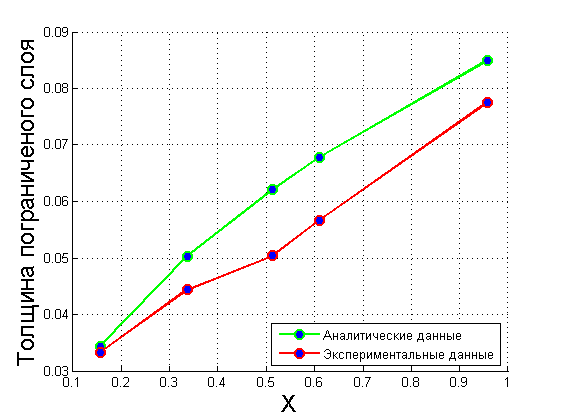
\includegraphics[width = \linewidth]{symm_pogr}}
    \captionof{figure}{Толщина погран. слоя (symmetry)}
  \end{minipage}
  \hfill
  \begin{minipage}[b]{0.5\linewidth}
  \center{\small Таб. 1: Толщина погран. слоя (symmetry).}\\ \quad \\
    \begin{tabular}[h!]{c|c|c|cc}
    $X$ & $V_{max}$ & $0.99 \cdot V_{max}$ & $\delta_{99} = Y_{x}$ & $\delta_{99}$ \ntb
    \hline  
    $0.07L$ & 1.05 & 1.04 & 0.0387 & 0.0344 \ntb
    \hline
    $0.26L$ & 1.07 & 1.06 & 0.0444 & 0.0503 \ntb
    \hline
    $0.46L$ & 1.09 & 1.08 & 0.0504 & 0.0621 \ntb
    \hline
    $0.57L$ & 1.10 & 1.09 & 0.0567 & 0.0678 \ntb
    \hline
    $0.95L$ & 1.12 & 1.11 & 0.0775 & 0.0849 \ntb
    \end{tabular}
  \end{minipage}
\end{minipage}

\n\n  
\subsubsection{Верхняя граница outlet}

\begin{minipage}{\linewidth}
  \begin{minipage}{0.5\linewidth}
    \center{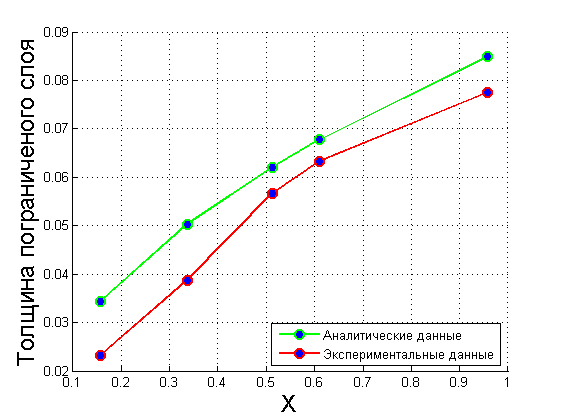
\includegraphics[width = \linewidth]{outlet_pogr}}
    \captionof{figure}{Толщина погран. слоя (outlet)}
  \end{minipage}
  \hfill
  \begin{minipage}[b]{0.5\linewidth}
  \center{\small Таб. 2: Толщина погран. слоя (outlet).}\\ \quad \\
    \begin{tabular}[h!]{c|c|c|cc}
    $X$ & $V_{max}$ & $0.99 \cdot V_{max}$ & $\delta_{99} = Y_{x}$ & $\delta_{99}$ \ntb
    \hline  
    $0.07L$ & 1.05 & 1.04 & 0.0232 & 0.0344  \ntb
    \hline  
    $0.26L$ & 1.05 & 1.04 & 0.0387 & 0.0503  \ntb
    \hline  
    $0.46L$ & 1.05 & 1.04 & 0.0567 & 0.0621  \ntb
    \hline  
    $0.57L$ & 1.05 & 1.04 & 0.0633 & 0.0678  \ntb
    \hline  
    $0.95L$ & 1.04 & 1.03 & 0.0775 & 0.0849  \ntb
    \end{tabular}
  \end{minipage}
\end{minipage}

\n\n
Для двух вариантов верхней границы расчетной области, экспериментальная толщина пограничного слоя несколько меньше ее аналитического значения.

\subsection{Профили скорости}
\subsubsection{Верхняя граница symmetry}

\begin{minipage}{\linewidth}
  \begin{minipage}{0.5\linewidth}
    \center{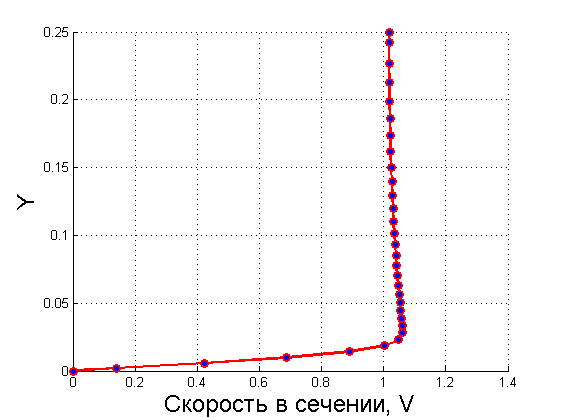
\includegraphics[width = \linewidth]{prof1_symm} \\ (a)}
  \end{minipage}
  \hfill
  \begin{minipage}{0.5\linewidth}
    \center{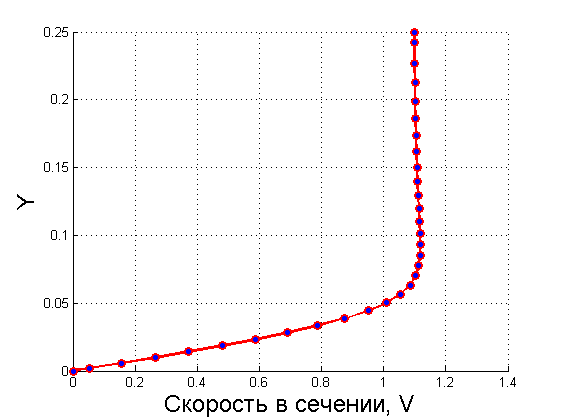
\includegraphics[width = \linewidth]{prof2_symm} \\ (б)}
  \end{minipage}
  \captionof{figure}{Профили скорости: (a) - сечение $X = 0.1L$, (б) - сечение $X = 0.95L$}
\end{minipage}

\n\n
\subsubsection{Верхняя граница outlet}
\begin{minipage}{\linewidth}
  \begin{minipage}{0.5\linewidth}
    \center{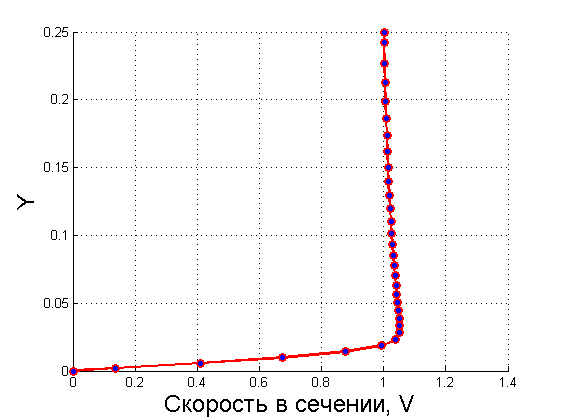
\includegraphics[width = \linewidth]{prof1_out} \\ (a)}
  \end{minipage}
  \hfill
  \begin{minipage}{0.5\linewidth}
    \center{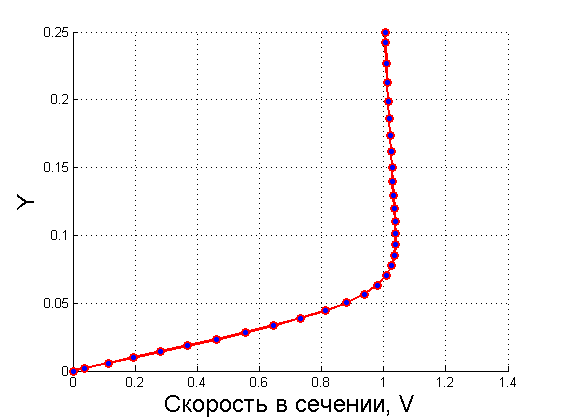
\includegraphics[width = \linewidth]{prof2_out} \\ (б)}
  \end{minipage}
  \captionof{figure}{Профили скорости: (a) - сечение $X = 0.1L$, (б) - сечение $X = 0.95L$}
\end{minipage}

\n
Профили скорости в начале пластины  близки друг к другу (рис. 10(а) и рис. 11(а)). Ближе к концу пластины максимальная скорость выше в эксперименте с граничным условием симметрии (рис. 10 (б)).

\subsection{Коэффициент поверхностного трения $C_f$}

\tabscale{1}

\begin{minipage}{\linewidth}
  \begin{minipage}{0.5\linewidth}
    \center{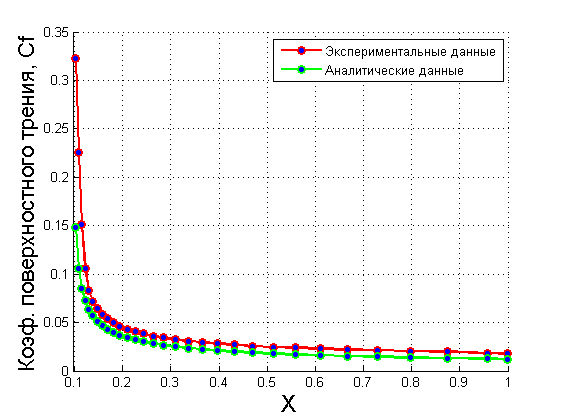
\includegraphics[width = \linewidth]{sk_sym} \\ (a)}
  \end{minipage}
  \hfill
  \begin{minipage}{0.5\linewidth}
    \center{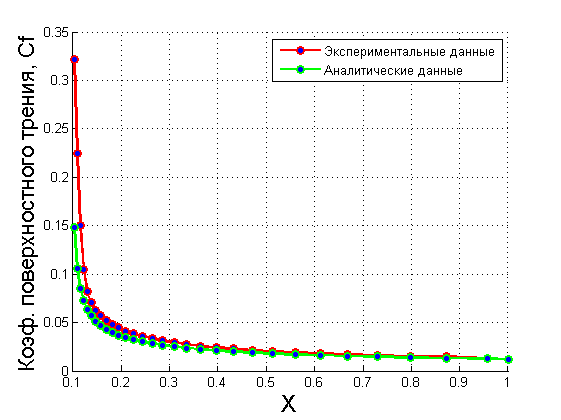
\includegraphics[width = \linewidth]{sk_out} \\ (б)}
  \end{minipage}
  \captionof{figure}{$C_f$ на пластине, верхняя граница: (a) - symmetry, (б) - outlet.}
\end{minipage}

\n\n
Экспериментальные значения коэффициента поверхностного трения близки к аналитическим в обоих случаях граничных условий расчетной области, но при граничном условии нормированного давления (рис. 12(б)) близость экспериментальные и аналитические данные ближе.

\n\n\noindent
$C_{f\text{эксп.}}$ -- экспериментальный коэффициент поверхностного трения.\\
$C_{f\text{ан.}}$ -- аналитический коэффициент поверхностного трения, полученный при помощи формулы Блазиуса $$C_f = \frac{0.664}{\sqrt{Re_x}}$$.

                                                                          
{\center{Таб. 3: Распределение коэффицента поверхностного трения, верхняя граница: \\ слева - symmetry, справа - outlet.}\\ \quad \\}
\begin{longtable}{>{\centering}p{2cm}|>{\centering}p{2cm}|>{\centering}p{2cm}p{2cm}>{\centering}p{2cm}|>{\centering}p{2cm}|>{\centering}p{2cm}}
  $X$    & $C_{f \,\text{эксп.}}$ & $C_{f \,\text{ан.}}$ & &  $X$  & $C_{f \,\text{эксп.}}$ & $C_{f \,\text{ан.}}$ \ntb
\cline{1-3} \cline{5-7}
0.1027 & 0.3226 & 0.0359 & & 0.1027 & 0.3212 & 0.0359\ntb
\cline{1-3} \cline{5-7}
0.1084 & 0.2260 & 0.0349 & & 0.1084 & 0.2246 & 0.0349\ntb
\cline{1-3} \cline{5-7}
0.1147 & 0.1516 & 0.0340 & & 0.1147 & 0.1503 & 0.0340\ntb
\cline{1-3} \cline{5-7}
0.1217 & 0.1059 & 0.0330 & & 0.1217 & 0.1046 & 0.0330\ntb
0.1293 & 0.0830 & 0.0320 & & 0.1293 & 0.0818 & 0.0320\ntb
\cline{1-3} \cline{5-7}
0.1378 & 0.0714 & 0.0310 & & 0.1378 & 0.0702 & 0.0310\ntb
\cline{1-3} \cline{5-7}
0.1470 & 0.0642 & 0.0300 & & 0.1470 & 0.0629 & 0.0300\ntb
\cline{1-3} \cline{5-7}
0.1572 & 0.0586 & 0.0290 & & 0.1572 & 0.0572 & 0.0290\ntb
\cline{1-3} \cline{5-7}
0.1684 & 0.0539 & 0.0280 & & 0.1684 & 0.0523 & 0.0280\ntb
\cline{1-3} \cline{5-7}
0.1807 & 0.0498 & 0.0271 & & 0.1807 & 0.0480 & 0.0271\ntb
\cline{1-3} \cline{5-7}
0.1942 & 0.0463 & 0.0261 & & 0.1942 & 0.0444 & 0.0261\ntb
\cline{1-3} \cline{5-7}
0.2091 & 0.0432 & 0.0251 & & 0.2091 & 0.0411 & 0.0251\ntb
\cline{1-3} \cline{5-7}
0.2255 & 0.0405 & 0.0242 & & 0.2255 & 0.0382 & 0.0242\ntb
\cline{1-3} \cline{5-7}
0.2436 & 0.0382 & 0.0233 & & 0.2436 & 0.0357 & 0.0233\ntb
\cline{1-3} \cline{5-7}
0.2634 & 0.0360 & 0.0224 & & 0.2634 & 0.0333 & 0.0224\ntb
\cline{1-3} \cline{5-7}
0.2852 & 0.0341 & 0.0215 & & 0.2852 & 0.0312 & 0.0215\ntb
\cline{1-3} \cline{5-7}
0.3092 & 0.0324 & 0.0207 & & 0.3092 & 0.0292 & 0.0207\ntb
\cline{1-3} \cline{5-7}
0.3356 & 0.0308 & 0.0198 & & 0.3356 & 0.0274 & 0.0198\ntb
\cline{1-3} \cline{5-7}
0.3646 & 0.0294 & 0.0190 & & 0.3646 & 0.0257 & 0.0190\ntb
\cline{1-3} \cline{5-7}
0.3966 & 0.0281 & 0.0182 & & 0.3966 & 0.0242 & 0.0182\ntb
\cline{1-3} \cline{5-7}
0.4317 & 0.0269 & 0.0175 & & 0.4317 & 0.0228 & 0.0175\ntb
\cline{1-3} \cline{5-7}
0.4704 & 0.0257 & 0.0167 & & 0.4704 & 0.0214 & 0.0167\ntb
\cline{1-3} \cline{5-7}
0.5129 & 0.0247 & 0.0160 & & 0.5129 & 0.0202 & 0.0160\ntb
\cline{1-3} \cline{5-7}
0.5597 & 0.0237 & 0.0154 & & 0.5597 & 0.0190 & 0.0154\ntb
\cline{1-3} \cline{5-7}
0.6111 & 0.0228 & 0.0147 & & 0.6111 & 0.0180 & 0.0147\ntb
\cline{1-3} \cline{5-7}
0.6677 & 0.0219 & 0.0141 & & 0.6677 & 0.0169 & 0.0141\ntb
\cline{1-3} \cline{5-7}
0.7299 & 0.0212 & 0.0134 & & 0.7299 & 0.0162 & 0.0134\ntb
\cline{1-3} \cline{5-7}
0.7984 & 0.0203 & 0.0128 & & 0.7984 & 0.0149 & 0.0128\ntb
\cline{1-3} \cline{5-7}
0.8737 & 0.0199 & 0.0123 & & 0.8737 & 0.0147 & 0.0123\ntb
\cline{1-3} \cline{5-7}
0.9566 & 0.0185 & 0.0117 & & 0.9566 & 0.0130 & 0.0117\ntb
\cline{1-3} \cline{5-7}
1.0000 & 0.0178 & 0.0115 & & 1.0000 & 0.0121 & 0.0115\ntb
\end{longtable}                                              
                     	                                                                         

\section{Анализ результатов с теплообменом}
\subsection{Распределение полей температуры}

\n\n
\pich{0.9}{3cm}{temp_pr_0_71}{Распределение скорости по оси $Ox$ ($Pr = 0.71$).}

\n\n
\pich{0.9}{3cm}{temp_pr_4_34}{Распределение скорости по оси $Ox$ ($Pr = 4.34$).}

Можно видеть, что толщина пограничного слоя тем больше, чем меньше число Прандтля.

\subsection{Толщина температурного пограничного слоя}

\n
\begin{minipage}{\linewidth}
  {\center{Таб. 4: Толщина температурного пограничного слоя при $Pr = 0.71$.}\\ \quad \\}
  \noindent
  \begin{center}
    \begin{tabular}{>{\centering}p{2cm}|>{\centering}p{2cm}|>{\centering}p{2cm}|>{\centering}p{2cm}|>{\centering}p{2cm}}
    $X$ & $\delta_{T99}$ & $\delta_{99}$ & $\frac{\delta_{T99}}{\delta_{99}}$ & $\frac{0.977}{\sqrt[3]{Pr}}$ \ntb
    \hline
    $0.07L$ & 0.0281 & 0.0387 & 1.2112 & \multirow{5}{*}{1.0952}\ntb
    \cline{1-4}
    $0.26L$ & 0.0567 & 0.0444 & 1.4651 & \ntb
    \cline{1-4}
    $0.46L$ & 0.0702 & 0.0504 & 1.2381 & \ntb
    \cline{1-4}
    $0.57L$ & 0.0775 & 0.1500 & 1.2243 & \ntb
    \cline{1-4}
    $0.95L$ & 0.1020 & 0.0775 & 1.3161 & \ntb
    \end{tabular}
  \end{center}
\end{minipage}

\n\n\noindent
\begin{minipage}{\linewidth}
  {\center{Таб. 5: Толщина температурного пограничного слоя при $Pr = 4.34$.}\\ \quad \\}
  \noindent\noindent\begin{center}
    \begin{tabular}{>{\centering}p{2cm}|>{\centering}p{2cm}|>{\centering}p{2cm}|>{\centering}p{2cm}|>{\centering}p{2cm}}
    $X$ & $\delta_{T99}$ & $\delta_{99}$ & $\frac{\delta_{T99}}{\delta_{99}}$ & $\frac{0.977}{\sqrt[3]{Pr}}$ \ntb
    \hline
    $0.07L$ & 0.0185 & 0.0387 & 0.7974 & \multirow{5}{*}{0.5990}\ntb
    \cline{1-4}
    $0.26L$ & 0.0333 & 0.0444 & 0.8605 & \ntb
    \cline{1-4}
    $0.46L$ & 0.0444 & 0.0504 & 0.7831 & \ntb
    \cline{1-4}
    $0.57L$ & 0.0504 & 0.1500 & 0.7962 & \ntb
    \cline{1-4}
    $0.95L$ & 0.0633 & 0.0775 & 0.8168 & \ntb
    \end{tabular}
  \end{center}
\end{minipage}

\n\n
Можно видеть, что экспериментальные значения толщины пограничного слоя несколько превосходят аналитические.

\subsection{Коэффициент теплоотдачи}

$Nu_{\text{эксп.}}$ -- экспериментальный коэффициент теплоотдачи (число Нуссельта).\\
$Nu_{\text{ан.}}$ -- аналитический коэффициент теплоотдачи, полученный при помощи формулы $$ Nu = \frac{1}{x} \cdot 0.332 \cdot \sqrt[3]{Pr} \cdot \sqrt{Re_x}.$$

\begin{longtable}{>{\centering}p{2cm}|>{\centering}p{2cm}|>{\centering}p{2cm}p{2cm}>{\centering}p{2cm}|>{\centering}p{2cm}|>{\centering}p{2cm}}
 $X$ & $Nu_{\text{эксп.}}$ & $Nu_{\text{ан.}}$ & & $X$ & $Nu_{\text{эксп.}}$ & $Nu_{\text{ан.}}$ \ntb
\cline{1-3} \cline{5-7}
0.1027 & 405.1925 & 213.7196 & & 0.1027 & 569.8913 & 390.7702\ntb
\cline{1-3} \cline{5-7}                                      
0.1084 & 181.0780 & 153.0478 & & 0.1084 & 416.5972 & 279.8364\ntb
\cline{1-3} \cline{5-7}                                      
0.1147 & 121.8102 & 123.3911 & & 0.1147 & 278.6900 & 225.6113\ntb
\cline{1-3} \cline{5-7}                                      
0.1217 & 101.5640 & 104.7008 & & 0.1217 & 193.3917 & 191.4375\ntb
\cline{1-3} \cline{5-7}                                      
0.1293 & 89.9789  & 91.6877  & & 0.1293 & 155.7378 & 167.6441\ntb
\cline{1-3} \cline{5-7}                                      
0.1378 & 80.5702  & 81.6581  & & 0.1378 & 139.2913 & 149.3056\ntb
\cline{1-3} \cline{5-7}                                      
0.1470 & 72.9729  & 73.8135  & & 0.1470 & 129.2160 & 134.9625\ntb
\cline{1-3} \cline{5-7}                                      
0.1572 & 66.6277  & 67.3042  & & 0.1572 & 120.2362 & 123.0607\ntb
\cline{1-3} \cline{5-7}                                      
0.1684 & 61.2884  & 61.8245  & & 0.1684 & 111.8149 & 113.0414\ntb
\cline{1-3} \cline{5-7}                                      
0.1807 & 56.7091  & 57.1190  & & 0.1807 & 104.1007 & 104.4377\ntb
\cline{1-3} \cline{5-7}                                      
0.1942 & 52.7237  & 53.0173  & & 0.1942 & 97.1815  & 96.9382 \ntb
\cline{1-3} \cline{5-7}                                      
0.2091 & 49.1940  & 49.3784  & & 0.2091 & 90.9736  & 90.2846 \ntb
\cline{1-3} \cline{5-7}                                      
0.2255 & 46.0472  & 46.1277  & & 0.2255 & 85.4023  & 84.3411 \ntb
\cline{1-3} \cline{5-7}                                      
0.2436 & 43.2122  & 43.1926  & & 0.2436 & 80.3538  & 78.9744 \ntb
0.2634 & 40.6628  & 40.5464  & & 0.2634 & 75.7888  & 74.1360 \ntb
\cline{1-3} \cline{5-7}                                      
0.2852 & 38.3402  & 38.1298  & & 0.2852 & 71.6073  & 69.7174 \ntb
\cline{1-3} \cline{5-7}                                      
0.3092 & 36.2139  & 35.9121  & & 0.3092 & 67.7605  & 65.6625 \ntb
\cline{1-3} \cline{5-7}                                      
0.3356 & 34.2603  & 33.8697  & & 0.3356 & 64.2118  & 61.9283 \ntb
\cline{1-3} \cline{5-7}                                      
0.3646 & 32.4604  & 31.9841  & & 0.3646 & 60.9303  & 58.4805 \ntb
\cline{1-3} \cline{5-7}                                      
0.3966 & 30.7885  & 30.2296  & & 0.3966 & 57.8724  & 55.2725 \ntb
\cline{1-3} \cline{5-7}                                      
0.4317 & 29.2395  & 28.6021  & & 0.4317 & 55.0307  & 52.2967 \ntb
\cline{1-3} \cline{5-7}                                      
0.4704 & 27.7927  & 27.0806  & & 0.4704 & 52.3702  & 49.5149 \ntb
\cline{1-3} \cline{5-7}                                      
0.5129 & 26.4414  & 25.6607  & & 0.5129 & 49.8769  & 46.9187 \ntb
\cline{1-3} \cline{5-7}                                      
0.5597 & 25.1767  & 24.3293  & & 0.5597 & 47.5409  & 44.4843 \ntb
\cline{1-3} \cline{5-7}                                      
0.6111 & 23.9822  & 23.0818  & & 0.6111 & 45.3242  & 42.2033 \ntb
\cline{1-3} \cline{5-7}                                      
0.6677 & 22.8734  & 21.9080  & & 0.6677 & 43.2699  & 40.0571 \ntb
\cline{1-3} \cline{5-7}                                      
0.7299 & 21.7937  & 20.8041  & & 0.7299 & 41.2567  & 38.0388 \ntb
\cline{1-3} \cline{5-7}                                      
0.7984 & 20.8284  & 19.7626  & & 0.7984 & 39.4507  & 36.1344 \ntb
\cline{1-3} \cline{5-7}                                      
0.8737 & 19.8413  & 18.7806  & & 0.8737 & 37.6355  & 34.3389 \ntb
\cline{1-3} \cline{5-7}                                      
0.9566 & 18.9712  & 17.8524  & & 0.9566 & 35.9763  & 32.6417 \ntb
\cline{1-3} \cline{5-7}                                      
1.0000 & 18.5233  & 17.4182  & & 1.0000 & 35.1222  & 31.8479 \ntb
\end{longtable}                                              
                           

Можно видеть, что экспериментальные значения коэффициента теплоотдачи в начале пластины больше аналитических, но при удалении от начала пластины значения становятся близки друг к другу.

\section{Вывод}
В ходе работы были проведены сравнения толщины пограничного слоя при различных граничных условиях верхней границы рассчетной области. В эксперименте с теплообменом было проанализированно как влияет число Прандтля на толщину пограничного слоя и на распределение коэффициента теплоотдачи на подогреваемой пластине. В целом, экспериментальные значения во всех опытах были близки к аналитическим.
\end{document}	
